%%-*- mode: LaTeX; mode: FlySpell; -*-

\section{Abstraction with Agents}  \label{sec:agents-abstraction}

\comment{outer border should be ``boundary'' in this section. }

Having laid the foundations for abstraction on the core $\guEA$ model, extending grouping to a model that also includes agents, the third pillar of the PROV model, is quite straightforward. Agents may be humans or software systems. 
%
Specifically, we now consider the node type $\ag$ and the following additional relation types from the PROV schema of Sec.~\ref{sec:prov-core}:

\begin{eqnarray*}
\waw      & \subseteq & \act \times \ag \\
\attrTo   & \subseteq & \en \times \ag \\
\delegate & \subseteq & \ag \times \ag  
\end{eqnarray*}
% \begin{align*}
% \waw \subseteq \act \times \ag \\
% \attrTo \subseteq \en \times \ag \\
% \delegate \subseteq \ag \times \ag  
% \end{align*}
% %Instances of this extended model now include the three relation types above.
%$\{\attrTo(e,ag)|e \in \en, ag \in \ag\} \cup \{\waw(a,ag)|a \in \act, ag \in \ag\} \cup \{ \delegate(ag_1, ag_2) | ag_1, ag_2 \in \ag\}$. 
%

We use the shorthand relation names $\waw$,  $\attrTo$ and $\delegate$  for \textit{wasAssociatedWith},  \textit{wasAttributedTo} and \textit{actedOnBehalfOf}. These denote responsibility of an agent for an activity ($\waw$), responsibility of an agent for an entity ($\attrTo$), and delegation between two agents ($\delegate$). 
%

Note that PROV admits an additional optional activity element to $\delegate$, which is used to  qualify the delegation as occurring within the scope of that activity. For simplicity, we are not going to consider this qualified version of the relation.
%
Thus, we can still assume that these new relations are binary, and so we continue to view an instance of a provenance graph as a directed graph $G=(V,E)$, where new $V= \en ~\cup~ \act ~\cup~ \ag$, and where each relation instance maps to a labelled directed edge.  We denote the set of all such graphs as $\guaEAG$.

The main implications of adding agents to our abstraction model are that (i) a new \textit{ag-grouping} operator must be introduced, and (ii) the existing definitions of e-grouping and a-grouping must be modified slightly. 

In order to incorporate agents into the definition of $\group$, observe that, for all three relations involving agents, the agent node is always the \textit{target} of the directed edge.
%
This means that agents can be viewed as part of an ``outer layer'' in the provenance graph.
%
This is illustrated in Fig.~\ref{fig:agents-baseline}, where the agent nodes and new relations are shown in bold lines in the outer side of the digraph.

\begin{figure}
\centering
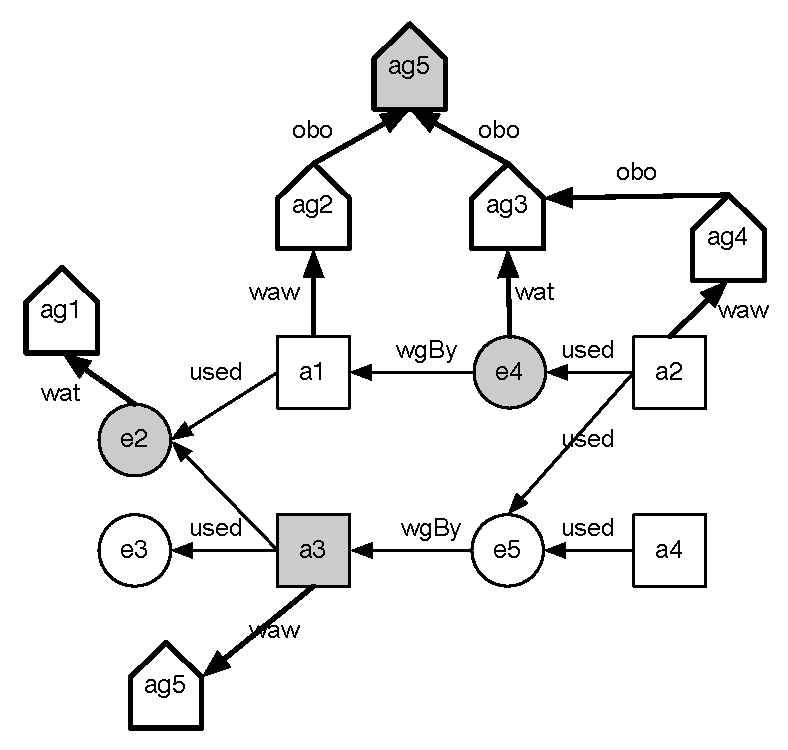
\includegraphics[scale=.5]{figures/agents-baseline}
\caption{$\guaEAG$ provenance graph. Agents lie on the outer border of the digraph. Shaded nodes show a possible grouping set in the general case.}  \label{fig:agents-baseline}
\end{figure}

This observation suggests we can break down the analysis of grouping with agents into the following three parts.
%
\begin{enumerate}
\item $V_{gr} \subset \ag$. This is the case for ag-grouping, which only involves the outer layer of the graph. Since agents are only related to each other through delegation: $\delegate(ag_1 , ag_2)$, grouping in this case is akin to \textit{homogeneous grouping} from Sec.~\ref{sec:closure}, \jwb{ in the sense that} no nodes of other types are ever involved, and $v_{new} \in \ag$. %\comment{this is NOT what type-homogeneity means. Nodes of other types ARE (or at least can) involved there, because of $\pclos$. }

\item $V_{gr} \subset \en \cup \act$ as in Sec.~\ref{sec:grouping}. This is the case of t-grouping (Def.~\ref{def:t-grouping}), where the nodes involved in the abstraction are in the inner layer, but they may be related to agent nodes via $\waw$ and $\wat$ relations.

\item $V_{gr} \subset \en \cup \act \cup \ag$.  Here, the group set may contain any combination of nodes. However, the peripheral role played by agents relative to entities and activities suggests that it may be reasonable to restrict this case to e-grouping or a-grouping, i.e., a combination of node types may include agents, but it should not be abstracted by a new agent node.
%
\end{enumerate}



\subsection{Ag-grouping: abstracting agents}  \label{sec:ag-grouping}

We begin with the case where abstraction is performed over a set of agents, i.e., $V_{gr} \subset \ag$.
%
In this case, the existing definition of t-grouping (Def.~\ref{eq:t-grouping}) extends naturally to $\guaEAG$ graphs.
%
%
T-grouping involves three operators: $\clos$, $\extend$, and $\repl$.
%
Since $\clos(V_{gr}, \jwb{G})$ operates only on $\delegate$ relations, it follows that its result is also homogeneous, i.e., $\clos(V_{gr}, \jwb{G}) \subset \ag$. Also, there is no need to restore type validity by extending the closure, i.e., $\extend$ is the identity: $\extend(\clos(V_{gr},  \jwb{G}), V, \ag) = \clos(V_{gr},  \jwb{G})$.
%
Finally, it is easy to see that our original definition of group replace (Def.~\ref{def:group-replace}) is general enough to accommodate the ``rewiring'' of the new abstract agent node. 
%
We illustrate this informally using the patterns of Fig.~\ref{fig:d-chains-abstracted}.
%

In pattern (a), $V_{gr} = \{ ag_1, ag_4 \}$, and $\clos(V_{gr},  \jwb{G}) =  \{ ag_1, ag_2, ag_3, ag_4 \}$.
%
In this case, the closure includes all the intermediate agents in the delegation chain between $ag_1$ and $ag_4$.
%
Replacement trivially transforms $G$ into the single abstract agent $ag_N$.


\begin{figure}
\centering
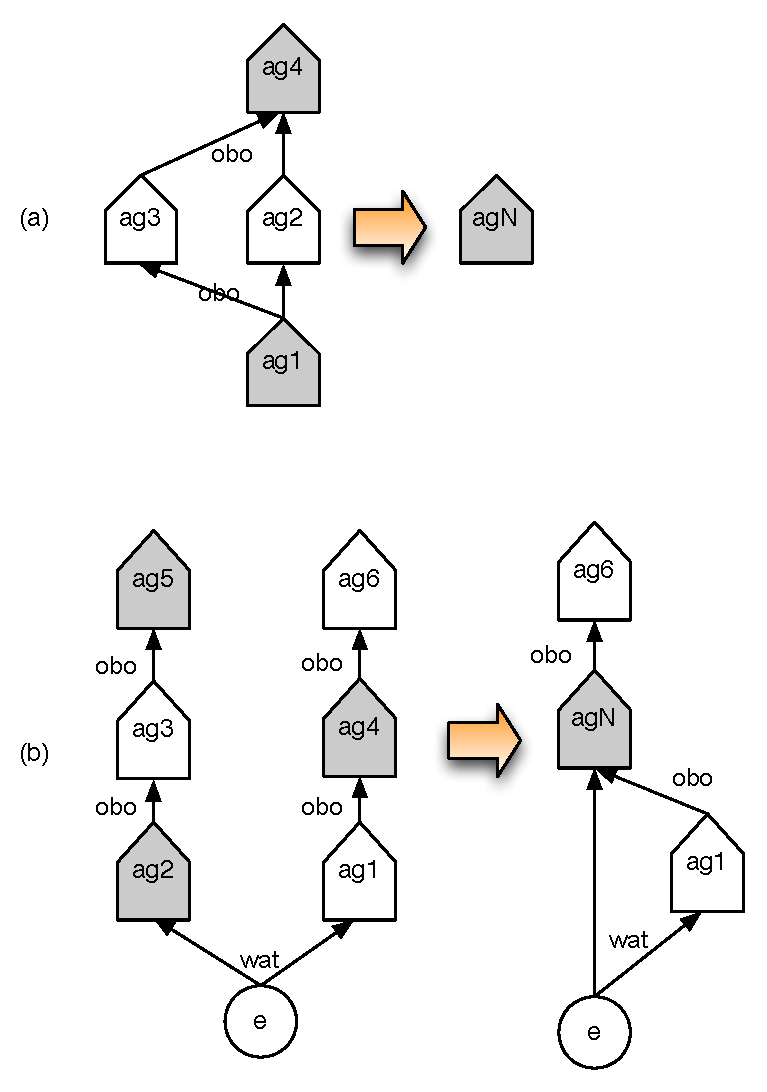
\includegraphics[scale=.5]{figures/d-chains-abstracted}
\caption{ag-grouping involving delegation.}
\label{fig:d-chains-abstracted}
\end{figure}

In pattern (b), $V_{gr} = \{ ag_2, ag_5, ag_4 \}$.
%
Note that not all agent nodes in $V_{gr}$ are related, either directly or through a path. This is not a problem, as we have $V_{clos} = \clos(V_{gr},  \jwb{G}) =   \{ ag_2, ag_5, ag_4, ag_3 \}$. Replacement applies as follows, where $\vartheta_{int}(V_{clos})$ is the set of relations beginning and ending inside $V_{clos}$:
\begin{eqnarray*}
\vartheta_{int}(V_{clos}) & = & \{ \delegate(ag_2, ag_3), \delegate(ag_3, ag_5) \} \\
\vartheta_{in}(V_{clos}) & = & \{ \wat(e, ag_2), \delegate(ag_1, ag_4) \} \\
\vartheta_{out}(V_{clos}) & = & \{ \delegate(ag_4, ag_6) \}
\end{eqnarray*}

% \begin{align*}
% &\vartheta_{int}(V_{clos}) = \{ \delegate(ag_2, ag_3), \delegate(ag_3, ag_5) \} \\
% &\vartheta_{in}(V_{clos}) = \{ \wat(e, ag_2), \delegate(ag_1, ag_4) \} \\
% &\vartheta_{out}(V_{clos}) = \{ \delegate(ag_4, ag_6) \}
% \end{align*}
% \

%
Thus, $\repl(V_{clos}, ag_N, G)$ maps relations in the original graph to those in the abstracted graph as follows:
%
\begin{eqnarray*}
\delegate(ag_4, ag_6) & \rightarrow &  \delegate(ag_N, ag_6) \\
\wat(e, ag_2) & \rightarrow &  \wat(e, ag_N) \\
\delegate(ag_1, ag_4) & \rightarrow &   \delegate(ag_1, ag_N)
\end{eqnarray*}

% \begin{align*}
% &\delegate(ag_4, ag_6) \rightarrow \delegate(ag_N, ag_6) \\
% &\wat(e, ag_2) \rightarrow \wat(e, ag_N) \\
% &\delegate(ag_1, ag_4) \rightarrow  \delegate(ag_1, ag_N)
% \end{align*}
% %
In practice, replacement preserves agents $ag_1$ and $ag_6$ and restores their delegation relations relative to the new abstract agent, $ag_N$. It also maps relation $\wat(e,ag_2)$, which involves the untouched $e$ node, to a new relation of the same type: $\wat(e,ag_N)$. 

We conclude that, in this first case, Def.~\ref{def:homo-group} applies without changes.

%\mnote{
%Points we must include somewhere
%\begin{itemize}
%  \item $V_{ag}$ means only type ag nodes included..
%  \item short forms of relations for general use
%  \item $\delegate(a,b) \in E$ means $(a,b) \in E \land label(a,b) = \delegate$
%  \item like-for-like: agents are abstracted to agents, not anything else.
%\end{itemize}
%}\\
%\mnote{
%  \begin{itemize}
%  \item close all delegate chains up, so we avoid cycles. ref sec on path closure.
%  \item remove and replace with $v_{new}$. 
%  \item rewire graph
%    \begin{itemize}
%    \item $\delegate$: agnets can't delagate to themselves \fbox{PM?}, otherwise retain delegate links
%    \item $\waw$ and $\wat$ remove all links: replace those that cross the abstract node boundary
%    \end{itemize}
%  \end{itemize}
%}
%

\subsection{a-grouping and e-grouping with agents}  \label{sec:t-grouping-agents}

The second case, where $V_{gr} \subset \en ~\cup~ \act$, is t-grouping with added agents relations.
%
Here the $\repl$ operator (Def.~\ref{def:group-replace}) must now consider how edges that involve agents are mapped to new edges in the abstract graph. 
%
We have already observed that agent nodes are always the targets of directed edges.
%
It follows that the closure of a set of nodes $V_{gr} \subset \en \cup \act$ never adds agent nodes to $V_{gr}$, because this would require the added agent to be on a path between two nodes from $\en ~\cup~ \act$, and therefore to be the source of a directed edge. 
%
%there can be no paths of the form $x \leftarrow ag \leftarrow y$  for $x,y \in \en \cup \act$.

%
A second observation is that if $\waw(a, ag)$ holds, and $a$ is involved in a-grouping, then $a$ is replaced by $a_{new}$, and thus $\waw(a_{new}, ag)$ also holds (Fig.~\ref{fig:agents-relations-patterns}(a1)).
%
Similarly for e-grouping, if $\wat(e, ag)$ holds, and $e$ is involved in e-grouping, then $e$ is replaced by $e_{new}$, and $\wat(e_{new}, ag)$ holds  (Fig.~\ref{fig:agents-relations-patterns}(b1)).
%
On the other hand, suppose $\waw(a,ag)$ holds and e-grouping is performed. A simple case is shown in Fig.~\ref{fig:agents-relations-patterns}(c1).
%
In this case, $a$ is replaced by $e_{new} \in \en$, therefore $\waw(e_{new},ag)$ is type-incorrect. Similarly, $\wat(e,ag)$ after a-grouping would become, incorrectly,  $\wat(a_{new}, ag)$.
%
These two patterns are summarised in Fig.~\ref{fig:agents-relations-patterns}(a2, b2 resp.). Note that one cannot simply replace association with attribution, i.e., replace relation $\waw(a, ag)$ with $\wat(e_N, ag)$, because there is no guarantee that any of the entities represented by the new $e_N$ had been attributed to $ag$ in the original graph. Similarly, one cannot replace $\wat(e, ag)$ with $\waw(a_N, ag)$.
%
Instead, in pattern (a) we simply remove the incorrect $\waw$ relations following e-grouping, and similarly, in pattern (b) we remove the incorrect $\wat$ relations following a-grouping.

\begin{figure}
\centering
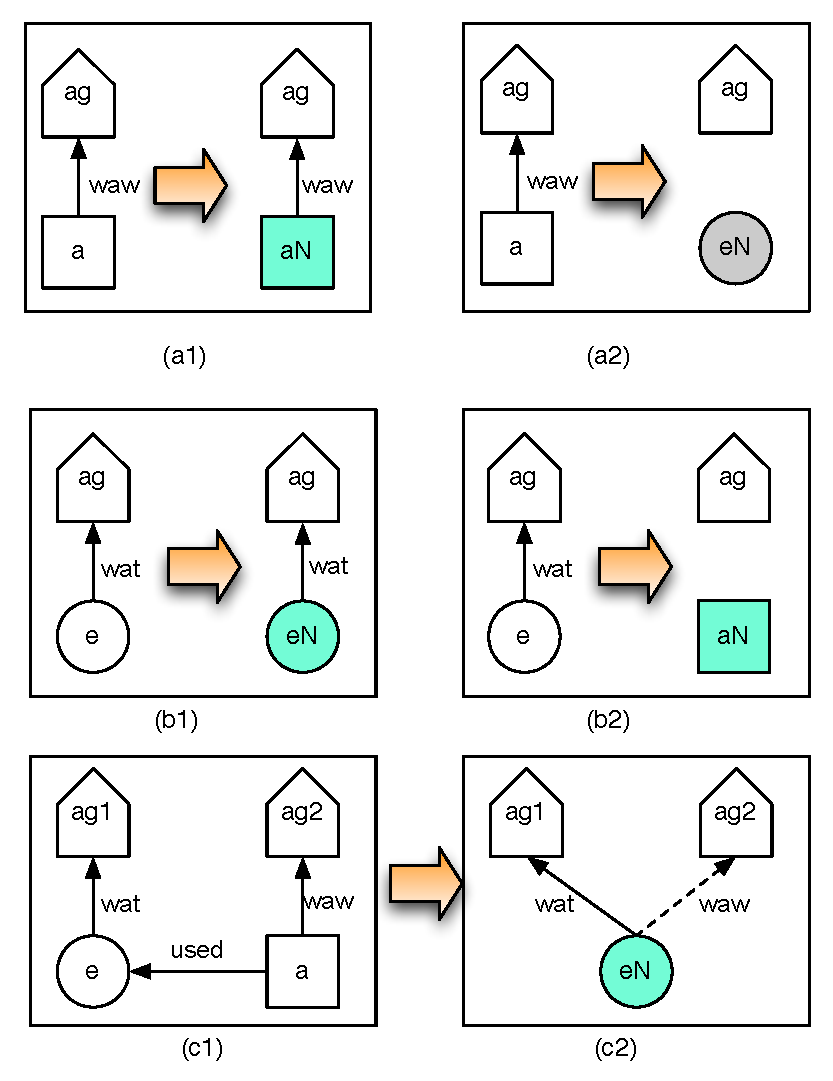
\includegraphics[scale=.5]{figures/agents-relations-patterns}
\caption{$\waw$ and $\wat$ edges involving nodes in $\clos(V_{gr},G)$ may need to removed following e-grouping and a-grouping, respectively.}  \label{fig:agents-relations-patterns}
\end{figure}

%
These considerations suggest that the definition of the $\repl$ function for grouping needs to be adapted for the case where agents are involved. 
%
To understand why, recall from Sec.~\ref{sec:closure} that $\repl$ replaces a type-homogeneous set, computed by the $\extend$ function, with an abstract node of the same type. An extension of type $t$ augments the closure of a grouping set by adding all adjacent nodes of the same type to it. This ensures that replacing the nodes in the extension with an abstract node of the same type preserves the type correctness of the relations. 
%
However it should be clear from the example above (parts c1, c2 of the figure), that both e-grouping and a-grouping on the set  $V_{gr} = \{ a, e\}$  result in one of the two agent relations being incorrect. Intuitively, this is because the extension function fails to incorporate agents, leaving the agent relations exposed on the outcut of $V_{gr}$ (in fact, $\extend$ in this example does nothing at all).

The pattern in (c2) (or its symmetric, for a-grouping), can be obtained simply by ensuring that $\repl$ deletes the incorrect relations.
%
The following variation on Definition~\ref{def:eq:outcut} ensures these deletions are enforced.
\begin{align*}
\vartheta_{out}'(V_{gr}') = \{ & v \xleftarrow{t}  v_{new} |  v \xleftarrow{t} v' \in \vartheta_{out}(V_{gr}') ~\wedge \\
      ( & (t = \wat \wedge \type(v_{new}) = \en) ~\vee \\
        & (t = \waw \wedge \type(v_{new}) = \act)  ~\vee \\
        & (t \neq \wat \wedge t \neq \waw) )\} 
\end{align*}


%Agents may also be abstracted. Here, a naive approach raises again the problem of cycles in the graph.   To illustrate, suppose the agents $ag2$, $ag4$ and $ag5$ are to be abstracted from the two delegation chains in Figure~\ref{fig:d-chains-abstracted}. 
%
%
% 
%
%This leads to agent $ag3$ both delegating to and being a delegate of the abstract agent node $a''$, a situation which we disallow 
%
%\mnote{
%@PM there doesn't seem to be  a constraint that excludes this.  Should we disallow it?  Why/Why not?
%}
%
% 
%We introduce \emph{delegation chain closure}, which is akin to path closure and includes   agents which, although not part of the original request, must also be abstracted. 
%
%\begin{definition}[Delegate Chains]
%\label{def:del-chain}
%A \emph{delegate chain} is a directed chain of agents $a_1,a_2,\ldots,a_n$, such that $\forall i<n\spot \delegate(a_i,a_{i+1}) \in E$. 
%\end{definition}
%
%
%In Figure~\ref{fig:d-chains-abstracted}, agent $ag3$ must be included in the path.  The function $\dclos$, given in Definition~\ref{def:dclos}, is the result of restricting function $\clos$ (Definition~\ref{def:clos}) to operate only on agents and traverse only $\delegate$ links.
% 
%\begin{definition}[Delegate Chain Closure]
%\label{def:dclos}
%Let $G = (V,E) \in \guaEAG$ be a provenance graph, and let $V_{ag} \subset V$ be a set of agents.   
%For each pair  $a_i, a_j \in V_{ag}$ such that there is a delegate chain beginning at  $a_i$ and ending at $a_j$,  let $V_{ij} \subset V$ be the set of all nodes in the chain.
%The \emph{delegate chain closure} of $V_{gr}$ in $G$ is 
%\[\dclos(V_{ag}, G)  =  \bigcup_{v_i, v_j \in V_{ag}} V_{ij} \]
%\end{definition}
%
%
%For any set of agents $V_{ag}$ to be abstracted, $\dclos(V_{ag},G)$ returns the set of agents which need to be replaced by a new abstract agent.  Replacing these agents is again a similar task to the one carried out by the $\repl$ operator.
%
%
%\begin{definition}[Agents Replace]
%\label{def:agent-replace}
%\[ \agrepl(V_{ag}, ag_{abs}, G) = (V', E'), \mbox{ where: }\]
%\begin{align*}
%V' & = V \setminus V_{ag}  \cup \{ag_{abs}\} \\
%E' & = E \setminus & \\
%   & \{ \delegate(ag_{abs},ag)  | \\
%   & \quad  \exists ag' \in V_{ag} \spot ag \in V\hide V_{ag} \\
%   & \quad \land  \delegate(ag',ag) \in E \} \\
%   & \cup \{ \delegate(ag,ag_{abs})  | \\
%   & \quad \exists ag' \in V_{ag} \spot ag \in V\hide V_{ag} \land  \\
%   & \quad \delegate(ag,ag') \in E \} \\
%   & \cup \{ \waw(a,ag_{abs})| \\
%   & \quad \exists ag'\in V_{ag}\spot \waw(a,ag') \in E\}\\
%   & \cup \{ \wat(e,ag_{abs})| \\
%   & \quad \exists ag'\in V_{ag}\spot \wat(e,ag') \in E\}\\
%\end{align*}
%\end{definition}
%
%
%This definition replaces all relations between agents in the set $V_{ag}$ and agents in $V\hide V_{ag}$, and therefore we cannot create  orphan agents using $\agrepl$. 
%
%
%\begin{definition}[Grouping Agents]
%\label{def:ag-group-by}
%\begin{align*}
%\aggroup(G,V_{ag},ag_{abs}) = \agrepl(\dclos(V_{ag},G),ag_{abs},G) 
%\end{align*}
%
%\end{definition}


\subsection{The general case: grouping on any node type}

The third and more general case, where \mbox{$V_{gr} \subset \en ~\cup~ \act ~\cup~ \ag$}, presents one further  difficulty. Consider performing e-grouping on the pattern of Fig.~\ref{agents-baseline-obo-problem} (left), with \mbox{$V_{gr} = \{ e_4, ag_5 \}$}.
%
We have \mbox{$\clos(V_{gr}, \jwb{G}) = \{ e_4, ag_5, ag_3 \}$}, resulting in the abstraction on the right.
%
Clearly, the former $\delegate(ag_4, ag_3)$ relation should not be mapped in the final graph. 
%
This issue arises because there the extension function, which guarantees type consistency for e- and a-nodes, does not include agents. 
%

Once again we deal with the issue by changing the definition of $\repl$ to ensure that the incorrect relation is not mapped. 
%
Note that a change is required to $\vartheta_{in}'(V_{gr}')$ rather than $\vartheta_{out}'(V_{gr}')$ as in the previous case. The new definition is as follows.
\begin{align*}
\vartheta_{in}'(V_{gr}') = \{ & v_{new} \xleftarrow{t}  v |  v' \xleftarrow{t} v \in \vartheta_{in}(V_{gr}') \\
    & \wedge ( (t = \delegate \wedge \type(v_{new}) = \ag) \vee t \neq \delegate )\} 
\end{align*}
Thus, a delegation relation is mapped in the abstract graph only if the target abstract node is an agent.

\begin{figure}
\centering
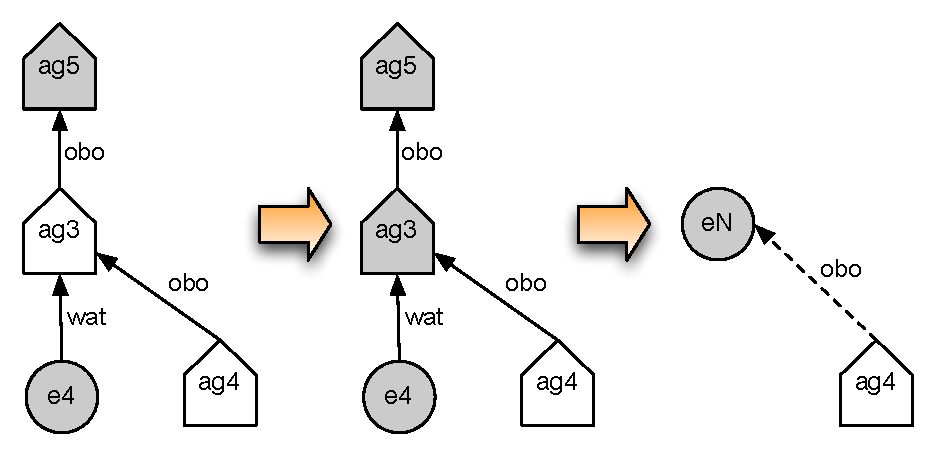
\includegraphics[scale=.5]{figures/agents-baseline-obo-problem}
\caption{e-grouping leads to incorrect $\delegate$ relation when agents are part of a closure.}
\label{agents-baseline-obo-problem}
\end{figure}

With the new version of the $\repl$ function, introduced in the previous two sections, some of the relations in the original graph $G$ are not mapped to the abstracted graph $G'$. This makes it possible for some of the nodes in $G'$ to end up disconnected from the rest of the graph. 
%
As an example, the graph in Fig.~\ref{agents-baseline-abstracted} shows the result of e-grouping over the shaded nodes in the graph of Fig.~\ref{fig:agents-baseline}. The combination of closure, extensions and replacement results in $ag_5$ being isolated, or ``orphaned'' in the abstract graph. 

%
As isolated agent nodes may not be significant to consumers of the abstracted graphs, for completeness we provide a simple function to optionally remove them at the end of the abstraction process, as follows.

\begin{figure}
\centering
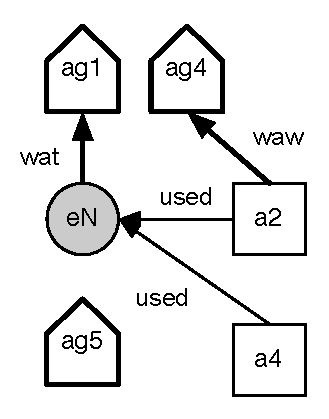
\includegraphics[scale=.5]{figures/agents-baseline-abstracted}
\caption{Abstracted version of the graph in Fig.~\ref{fig:agents-baseline} after e-grouping involving agents.}
\label{agents-baseline-abstracted}
\end{figure}


\begin{definition}[Removing isolated agents]
\label{def:orphanremove}
Let $G = (V,E) \in \guaEAG$, and 
\begin{align*}
 \mathit{isolated}(G) = \{  & v \in V | \type(v) = \ag \\
   & \wedge \nexists v' \in V . ((v',v) \in E \vee (v,v') \in E) \}
\end{align*}
Then:
\[ \remIsolated((V,E)) = (V \setminus \mathit{isolated}(G), E) \] 
\end{definition}


